\documentclass{article}
\usepackage{hyperref}
\usepackage{Style}

\nocite{*} % Comentar si quiero citar
%\addbibresource{bibliografia.bib} % Quitar el comentado si quiero usar bibliografia

\begin{document}

\begin{minipage}{2.5cm}
    \includegraphics[width=2cm]{imagen_puc.jpg}
\end{minipage}
\begin{minipage}{14cm}
    {\sc Pontificia Universidad Católica de Chile\\
    Facultad de Matemáticas\\
    Departamento de Matemática\\
    Profesor: Mauricio Bustamante -- Estudiante: Benjamín Mateluna}
\end{minipage}
\vspace{1ex}

{\centerline{\bf Topología Algebraica - MAT2850}
\centerline{\bf Tarea 1}}
\centerline{\bf 21 de agosto de 2025}

\section*{Problema 1}

\begin{lema}
    Sean $f_{0},f_{1}:X\to Y$ homotópicas y $g_{0},g_{1}:Y\to Z$ homotópicas, entonces 
    $g_{0}\circ f_{0}$ es homotópica a $g_{1}\circ f_{1}$.
\end{lema}
\begin{proof}
    Consideramos la función
    \begin{align*}
        H:X\times[0,1] &\to Z\htext{dada por} \\
        (x,t) &\to H_{g}(H_{f}(x,t),t)
    \end{align*}
    donde $H_{g}$ es una homotopía entre $g_{0}$ y $g_{1}$, similarmente para $H_{f}$. Notemos que
    \begin{equation*}
        H(x,0)=H_{g}(H_{f}(x,0),0)=g_{0}(f_{0}(x))=g_{0}\circ f_{0}(x)
    \end{equation*}
    análogamente, se tiene que $H(x,1)=g_{1}\circ f_{1}(x)$. Veamos que $H$ es continua, para ello
    tenemos el siguiente diagrama
    
    \vspace{2mm}
    \centerline{
        \xymatrixcolsep{3pc}\xymatrix{
            X\times[0,1] \ar[r]^-{id_{X}\times i} \ar@/_1.5pc/[rrr]_{H} & X\times[0,1]^{2} 
            \ar[r]^-{H_{f}\times id_{[0,1]}} & Y\times[0,1] \ar[r]^-{H_{g}} & Z
        }
    }
    \vspace{2mm}
    donde $i:[0,1]\to[0,1]^{2}$ esta dada por $i(t)=(t,t)$, que es continua por la propiedad 
    universal de la topología producto, de modo similar, el resto de funciones son continuas. Por 
    lo tanto, $H$ es continua, ya que corresponde a la composición de funciones continuas.
\end{proof}

\noindent Debemos probar tres puntos, que son los siguientes,
\begin{enumerate}
    \item Sea $X$ espacio topológico, veamos que $X\sim X$. Consideramos el homeomorfismo 
    $id_{X}:X\to X$, en particular, se tiene que $id_{X}\circ id_{X}=id_{X}$ es homotópica a 
    $id_{X}$ mediante la homotopía constante, luego $X\sim X$.

    \item Debemos verificar que si $X\sim Y$ entonces $Y\sim X$. Como $X\sim Y$, existe $f:X\to Y$
    equivalencia homotópica, sea $g:Y\to X$ su inversa homotópica. En particular, $g:Y\to X$ es
    continua y se cumple que $g\circ f\sim id_{Y}$ y $f\circ g\sim id_{X}$, es decir, $g$ es 
    equivalencia homotópica. Por lo tanto, $Y\sim X$.

    \item Sea $f:X\to Y$ una equivalencia homotópica y sea $f_{h}$ su inversa homotópica. 
    Consideramos $g:Y\to Z$ equivalencia homotópica. Afirmamos que $g\circ f:X\to Z$ es 
    equivalencia homotópica. En efecto, veamos que la función
    \begin{equation*}
        f_{h}\circ g_{h}:Z\to X
    \end{equation*}
    es equivalencia homotópica. Notemos, por el lema previo, que
    \begin{equation*}
        g\circ f\circ f_{h}\circ g_{h}\sim g\circ id_{Y}\circ g_{h}=g\circ g_{h}\sim id_{Z}
    \end{equation*}
    del mismo modo $f_{h}\circ g_{h}\circ g\circ f\sim id_{X}$. Concluimos que $X\sim Z$.
\end{enumerate}

\section*{Problema 2}
\noindent Para este problema diremos que $x\sim_{p}y$ si y solo si $[x]^{p}=[y]^{p}$, donde 
$[\cdot]^{p}$ es la componente conexa del punto. Esta relación resulta ser de equivalencia.

\begin{lema}
    Sea $h:X\to X$ con $h\sim id_{X}$, entonces $x\sim_{p}h_{x}$ para todo $x\in X$.
\end{lema}
\begin{proof}
    Sea $x\in X$. Como $h\sim id_{X}$, existe $H:X\times [0,1]\to X$ una homotopía entre $h$ e 
    $id_{X}$. Definimos la función $\gamma:[0,1]\to X$ dada por $\gamma(t):=H(x,t)$, que es 
    continua por la propiedad universal de la topología de subespacio. Así, $h(x)\in[x]^{p}$, lo
    que implica que $x\sim_{p}h(x)$.
\end{proof}

\noindent Sean $X\sim Y$, existe $f:X\to Y$ equivalencia homotópica y sea $g:Y\to X$ su inversa 
homotópica. Afirmamos que si $x\not\sim_{p}y$ entonces $f(x)\not\sim_{p}f(y)$. Supongamos que 
existen $x,y\in X$ tales que $x\not\sim_{p}y$ y $f(x)\sim_{p}f(y)$. Como $g$ es continua, tenemos
que $g(f(x))\sim_{p}g(f(y))$. Por el lema, resulta que
\begin{equation*}
    x\sim_{p}g\circ f(x)\sim_{p}g\circ f(y)\sim_{p}y
\end{equation*}
lo cual es una contradicción.

\vspace{2mm}
\noindent Lo anterior prueba que hay una inyección de las componentes arcoconexas de $X$ en las de
$Y$. Por simetría, vemos que también hay una inyección de las componentes arcoconexas de $Y$ en 
$X$, así, por cantor bernstein, ambos conjuntos estan en correspondencia uno a uno.

\vspace{2mm}
\noindent Notemos que $D^{1}$ es arcoconexo ya que es convexo, luego la cantidad de componentes 
componentes arcoconexas es uno. Por otro lado, veamos que $\{0,1\}$ no es conexo, pues la 
topología topología inducida es la discreta y por lo tanto hay dos componentes conexas. De este
modo, no existe equivalencia homotópica entre $D^{1}$ y $\s^{0}$.

\section*{Problema 3}
\begin{lema}
    Sea $A\subset\R^{2}$ un conjunto finito de puntos, entonces $X:=\R^{2}\setminus A$ es 
    arcoconexo.
\end{lema}
\begin{proof}
    Digamos que $A=\{x_{1},\cdots,x_{n}\}$. Como $A$ es finito, existe $\varepsilon>0$ tal que
    $B_{\varepsilon}(x_{i})\cap A=x_{i}$ para todo $1\leq i\leq n$. Sean $x,y\in X$, en $\R^{2}$
    consideramos el segmento de recta $L_{xy}:=\{(1-t)x+ty:t\in[0,1]\}$. Si 
    $L_{xy}\cap A=\emptyset$ es vacío, no hay nada que probar, supongamos que existe $i$ tal que
    $x_{i}\in L_{xy}\cap A$.

    \vspace{2mm}
    \noindent Sea $v\in(L_{xy}-x)\perp$ y definimos $L_{xy}^{*}:=\{tv+x_{i}:t\in\R\}$. Existe 
    $\delta>0$ tal que $\overline{B_{\delta}(x_{i})}\subseteq B_{\varepsilon}(x_{i})$, sean 
    $u,v\in L_{xy}\cap\partial B_{\delta(x_{i})}$ y $w\in L_{xy}^{*}\cap\partial 
    B_{\delta}(x_{i})$ que existen pues $L_{xy}\cap L_{xy}^{*}$ contienen a $x_{i}$, además 
    $u,v,w$ no son colineales ya que $L_{xy}\cap L_{xy}^{*}=x_{i}$.

    \vspace{2mm}
    \noindent Sean $t_{0}<t_{1}$ tales que $u=(1-t_{0})x+t_{0}y$ y $v=(1-t_{1})x+t_{1}y$. 
    Consideramos
    \begin{equation*}
        L=L_{xu}\cdot L_{uw}\cdot L_{wv}\cdot L_{vy}
    \end{equation*}
    donde $\cdot$ es la operación de concatenación. Como $t_{0}<t_{1}$, vemos que 
    $x_{i}\not\in L_{xu}\cup L_{vy}$. Además, como $u\in L_{xy}\cap L_{uw}$ y 
    $v\in L_{xy}\cap L_{wv}$, entonces $x_{i}\not\in L_{uw}\cdot L_{wv}$ y por convexidad resulta
    que
    \begin{equation*}
        L_{uw}\cdot L_{wv}\cap A=\emptyset
    \end{equation*}
    Si $(L_{xu}\cup L_{vy})\cap A=\emptyset$ entonces $L$ es el camino buscado, de lo contrario, 
    repetimos el procedimiento para cada punto en la intersección, por finitud, concluimos.

    \vspace{2mm}
    \begin{center}
        \begin{tikzpicture} %Ilustración de la demostración%
            \filldraw[color=black, fill=white, dashed] (0,0,0) circle (1.5);
            \filldraw[color=black, fill=white, thick] (0,0,0) circle (1);
            
            \coordinate (x_{i}) at (0,0);
            \coordinate (u) at ({-sqrt(2)/2},{-sqrt(2)/2});
            \coordinate (v) at ({sqrt(2)/2},{sqrt(2)/2});
            \coordinate (w) at (-{sqrt(2)/2},{sqrt(2)/2});

            \draw ($2*(u)$) -- ($2*(v)$);
            \draw (w) -- (x_{i});
            \draw (w) -- (u);
            \draw (w) -- (v);

            \filldraw (x_{i}) circle (1pt) node[anchor=north west]{$x_{i}$};
            \filldraw (u) circle (1pt) node[anchor=east]{$u$};
            \filldraw (v) circle (1pt) node[anchor=south]{$v$};
            \filldraw (w) circle (1pt) node[anchor=south]{$w$};
        \end{tikzpicture}
    \end{center}
    En la figura se muestra la situación.
\end{proof}

\noindent Sea $f\in\C[x_{1},\cdots,x_{n}]$, definimos $\mathbb{V}:=\{x\in\C^{n}:f(x)=0\}$. Notemos 
que
\begin{equation*}
    Conf_{n}(\C)=\C^{n}\setminus\bigcup_{i,j}\mathbb{V}(x_{i}-x_{j})
\end{equation*}
Sean $x,y\in Conf_{n}(\C)$, en $\C^{n}$ consideramos la recta $L_{xy}:=\{(x-y)z+y:z\in\C\}$, como
$\mathbb{V}(x_{i}-x_{j})$ es un hiperplano de dimensión $n-1$, se tiene que 
$L_{xy}\cap\mathbb{V}(x_{i}-x_{j})$ es vacío, un punto o $L_{xy}$. Dado que $x,y\in Conf_{n}(\C)$, 
vemos que $\abs{L_{xy}\cap\mathbb{V}(x_{i}-x_{j})}\leq1$, así
\begin{equation*}
    \abs{L_{xy}\cap\bigcup_{i,j}\mathbb{V}(x_{i}-x_{j})}\leq\sum_{i,j}\abs{L_{xy}
    \cap\mathbb{V}(x_{i}-x_{j})}\leq n^{2}
\end{equation*}
Notemos que $L_{xy}\cong\C$ con la identificación $w\to(x-y)w+y$, pero también $\C\cong\R^{2}$, 
entonces $L_{xy}\setminus\bigcup\mathbb{V}(x_{i}-x_{j})\cong\R^{2}\setminus A$ con $A$ un 
subconjunto finito.

\newpage
\section*{Problema 4}
\begin{enumerate}
    \item Sea $X=\R$ con la topología discreta. Supongamos, por contradicción, que existe $(K,f)$
    tales que $f:\abs{K}\to\R$ es homeomorfismo. Como $\abs{K}$ es segundo contable, pues 
    $\R^{\infty}$ es segundo contable, entonces $X$ es segundo contable, lo cual es una 
    contradicción. Claramente $X$ es Hausdorff.

    \item Probaremos un resultado previo.
    \begin{lema}
        Sea $X$ un espacio separable. Entonces todo conjunto discreto es numerable.
    \end{lema}
    \begin{proof}
        Sea $B\subseteq X$ un denso numerable. Sea $A\subseteq X$ un subconjunto discreto. Sea 
        $x\in A$, como $A$ es discreto, existe $U_{x}\subseteq X$ vecindad de $x$ tal que 
        $U_{x}\cap A=x$. Por densidad, existe $b_{x}\in U_{x}\cap B$. Definimos la función
        \begin{align*}
            f:A &\to B \\
            x &\to b_{x}
        \end{align*}
        Si $x\neq y$ entonces $U_{x}\cap U_{y}=\emptyset$, luego la función $f$ es inyectiva.
    \end{proof}

    \noindent Sea $X=\ell^{\infty}(\N)$ con la topología inducida por la norma. Sea 
    $S\subseteq\N$, definimos
    \begin{equation*}
        x_{S}=(x_{n})_{n}\hhtext{con}x_{n}:=\begin{cases}
            1 &\quad\text{ si }n\in S \\
            0 &\quad\text{ si no}
        \end{cases}
    \end{equation*}
    Consideramos $A=\{x_{S}:S\subseteq\N\}$, notemos que $A$ es no numerable y además si $S\neq T$ 
    se tiene que
    \begin{equation*}
        \norm{x_{S}-x_{T}}_{\infty}=1
    \end{equation*}
    es decir, $A$ es discreto, por el lema llegamos a una contradicción, lo que concluye el 
    resultado. Como $\ell^{\infty}(\N)$ es espacio métrico es Hausdorff.

    \item Demostraremos un lema previo.
    \begin{lema}
        Sea $K$ un complejo simplicial con finitos vértices. Entonces $\abs{K}$ es localmente 
        arcoconexo.
    \end{lema}
    \begin{proof}
        Sea $x\in\abs{K}$, existe $\varepsilon_{x}>0$, tal que
        \begin{equation*}
            B_{\varepsilon_{x}}(x)\cap\sigma\neq\emptyset\hhtext{entonces}x\in\sigma
            \text{, a saber}\hspace{4mm}\varepsilon_{x}:=\frac{1}{2}\min_{x\not\in\sigma}
            \{d(x,\sigma)\}
        \end{equation*}
        que está bien definido pues $K$ es finito. Sean $x\in\sigma$ y 
        $0<\varepsilon<\varepsilon_{x}$, como $\sigma$ y $B_{\varepsilon}(x)$ son convexos, 
        entonces $B_{\varepsilon}\cap\sigma$ es convexo, en particular, es arcoconexo. Luego,
        \begin{equation*}
            B_{\varepsilon}(x)\cap K=\bigcup_{x\in\sigma}B_{\varepsilon}\cap\sigma
        \end{equation*}
        es arcoconexo por ser unión de arcoconexos con $x$ un punto común. Consideramos
        \begin{equation*}
            \mathcal{B}:=\{B_{\varepsilon}(x):x\in\abs{K}\text{ y }0<\varepsilon<\varepsilon_{x}\}
        \end{equation*}
        Notemos que $\mathcal{B}$ es base y por lo dicho anteriormente cada abierto es arcoconexo.
    \end{proof}

    \noindent Consideremos el espacio
    \begin{equation*}
        X:=\overline{\left\{\left(x,sen\left(\frac{1}{x}\right)\right):x\in(0,1]\right\}}
    \end{equation*}
    conocido como el seno del topologo. Sabemos que $X$ es conexo, pero no es arcoconexo, y por 
    tanto no es localmente arcoconexo. Sea $(K,f)$ una triangulación de $X$ tal que $K$ es finito,
    entonces, por el lema, $\abs{K}$ es localmente arcoconexo, esto es una contradicción. Como $X$
    es subespacio de un espacio Hausdorff, entonces es Hausdorff.
\end{enumerate}

\newpage
\section*{Problema 5}
\noindent Debemos triangular tres espacios, que son los siguientes
\begin{enumerate}
    \item En $\R^{2}$ consideremos los puntos y los simplices
    \begin{equation*}
        \begin{matrix}
            v_{0}=(1,1) & v_{1}=(-1,1) \\
            v_{2}=-(1,1) & v_{3}=(1,-1)
        \end{matrix}
        \hspace{2cm}\begin{matrix}
            \sigma_{0}=\gen{v_{0},v_{1}} & \sigma_{1}=\gen{v_{1},v_{2}} \\
            \sigma_{2}=\gen{v_{2},v_{3}} & \sigma_{3}=\gen{v_{0},v_{3}}
        \end{matrix}
    \end{equation*}
    Como los puntos son distintos de a pares, los simplices están bien definidos, además es 
    sencillo verificar que $K=\bigcup_{i\geq0}\{\sigma_{i},v_{i}\}$ es un complejo simplicial.
    \begin{center}
        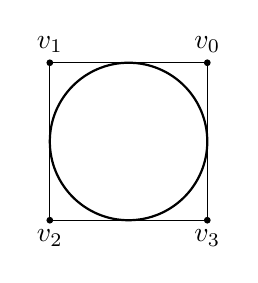
\begin{tikzpicture} %Triangulación del circulo
            \draw (1,1) -- (-1,1);
            \draw (1,1) -- (1,-1);
            \draw (-1,-1) -- (-1,1);
            \draw (-1,-1) -- (1,-1);

            \filldraw (1,1) circle (1pt) node[anchor=south]{$v_{0}$};
            \filldraw (-1,1) circle (1pt) node[anchor=south]{$v_{1}$};
            \filldraw (-1,-1) circle (1pt) node[anchor=north]{$v_{2}$};
            \filldraw (1,-1) circle (1pt) node[anchor=north]{$v_{3}$};

            \filldraw[color=black, fill=white, thick] (0,0) circle (1);
        \end{tikzpicture}
    \end{center}
    Afirmamos que $\abs{K}\cong\s^{1}$. Denotaremos por $\abs{\cdot}$ a la norma euclideana y 
    $\norm{\cdot}$ a la norma que corresponde a la norma del máximo. Consideramos la función 
    $f:\abs{K}\to\s^{1}$ dada por $f(x):=x/\abs{x}$ que resulta ser continua y esta bien definida 
    ya que $\abs{K}\subseteq\R^{2}\setminus\{0\}$. Afirmamos que $g:\s^{1}\to\abs{K}$ dada por 
    $g(x):=x/\norm{x}$ es la inversa de $f$ y es continua.

    \vspace{2mm}
    \noindent Notemos que $g$ esta bien definida puesto que 
    $\{x\in\R^{2}\setminus\{0\}:\norm{x}=1\}=\abs{K}$. Como $\norm{\cdot}$ y $\abs{\cdot}$ son 
    normas equivalentes, inducen la misma topología y por lo tanto $g$ es continua pues 
    $\s^{1}\subseteq\R^{2}\setminus\{0\}$. Luego,
    \begin{equation*}
        (f\circ g)(x)=f\left(\frac{x}{\norm{x}}\right)
        =\frac{\frac{x}{\norm{x}}}{\abs{\frac{x}{\norm{x}}}}=x
    \end{equation*}
    es decir, $f\circ g=id_{\s^{1}}$. Del mismo modo, $g\circ f=id_{\abs{K}}$. Lo que prueba que 
    $(K,f)$ es una triangulación de $\s^{1}$. Así, la característica de Euler de la triangulación
    es $V-E+F=4-4+0=0$.

    \item En $\R^{3}$ definimos los simplices y sus respectivos vértices
    \begin{equation*}
        \begin{array}{ll}
            v_{0}=(1,1,1) & v_{1}=(1,1,-1) \\
            v_{2}=(1,-1,-1) & v_{3}=(1,-1,1) \\
            v_{4}=(-1,1,1) & v_{5}=(-1,1,-1) \\
            v_{6}=(-1,-1,-1) &v_{7}=(-1,-1,1)
        \end{array}
        %
        \hspace{2cm}
        %
        \begin{array}{lll}
            \sigma_{0}=\gen{v_{0},v_{1},v_{3}} & \sigma_{1}=\gen{v_{1},v_{2},v_{3}} 
            & \sigma_{2}=\gen{v_{0},v_{3},v_{4}} \\
            \sigma_{3}=\gen{v_{0},v_{1},v_{4}} & \sigma_{4}=\gen{v_{1},v_{4},v_{5}} 
            & \sigma_{5}=\gen{v_{3},v_{4},v_{7}} \\
            \sigma_{6}=\gen{v_{4},v_{5},v_{7}} & \sigma_{7}=\gen{v_{5},v_{6},v_{7}} 
            & \sigma_{8}=\gen{v_{3},v_{6},v_{7}} \\
            \sigma_{9}=\gen{v_{2},v_{3},v_{6}} & \sigma_{10}=\gen{v_{1},v_{2},v_{6}} 
            & \sigma_{11}=\gen{v_{1},v_{5},v_{6}} \\
        \end{array}
    \end{equation*}
    Dado que los puntos $v_{i}$ no son colineales de a tres, vemos que cada $\sigma_{i}$ es un 
    simplice. Es sencillo ver que el conjunto $K$ formado por dichos simplices y sus respectivas 
    caras es un complejo simplicial.
    \begin{center}
        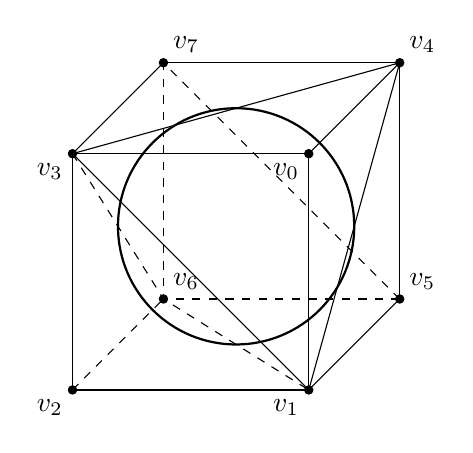
\begin{tikzpicture}[scale=1.5] %Triangulación de la esfera
            \filldraw[color=black, fill=white, thick] (0,0,0) circle (1);
            
            \coordinate (A) at (1,1,1);
            \coordinate (B) at (1,-1,1);
            \coordinate (C) at (-1,-1,1);
            \coordinate (D) at (-1,1,1);

            \coordinate (E) at (1,1,-1);
            \coordinate (F) at (1,-1,-1);
            \coordinate (G) at (-1,-1,-1);
            \coordinate (H) at (-1,1,-1);

            \draw (A) -- (B) -- (C) -- (D) -- cycle;
            
            \draw (H) -- (E) -- (F);
            \draw[dashed] (F) -- (G) -- (H);

            \draw (A) -- (E);
            \draw (B) -- (F);
            \draw[dashed] (C) -- (G);
            \draw (D) -- (H);

            \draw (D) -- (E) -- (B);
            \draw (B) -- (D);

            \draw[dashed] (D) -- (G) -- (B);
            \draw[dashed] (F) -- (H);

            \filldraw (A) circle (1pt) node[anchor=north east]{$v_{0}$};
            \filldraw (B) circle (1pt) node[anchor=north east]{$v_{1}$};
            \filldraw (C) circle (1pt) node[anchor=north east]{$v_{2}$};
            \filldraw (D) circle (1pt) node[anchor=north east]{$v_{3}$};
            
            \filldraw (E) circle (1pt) node[anchor=south west]{$v_{4}$};
            \filldraw (F) circle (1pt) node[anchor=south west]{$v_{5}$};
            \filldraw (G) circle (1pt) node[anchor=south west]{$v_{6}$};
            \filldraw (H) circle (1pt) node[anchor=south west]{$v_{7}$};
        \end{tikzpicture}
    \end{center}
    
    Afirmamos que $\abs{K}\cong\s^{2}$. Del mismo modo que antes definimos la función continua 
    $f:\abs{K}\to\s^{2}$ dada por
    \begin{equation*}
        f(x):=\frac{x}{\abs{x}}
    \end{equation*}
    con inversa continua $g:\s^{2}\to\abs{K}$ dada por
    \begin{equation*}
        g(x):=\frac{x}{\norm{x}}
    \end{equation*}
    donde $\abs{\cdot}$ y $\norm{\cdot}$ son la norma euclideana y la norma del máximo 
    respectivamente. Concluimos que $(K,f)$ es una triangulación de $\s^{2}$ cuya característica
    de Euler es $V-E+F=8-18+12=2$.

    \item Consideramos los puntos
    \begin{equation*}
        \begin{array}{lll}
            v_{0}=(1,0,0) & u_{0}=(-1,0,0) & w_{0}=(0,1,0) \\
            v_{1}=(2,-\frac{1}{2},1) & u_{1}=(-2,-\frac{1}{2},1) & w_{1}=(0,2,1) \\
            v_{2}=(2,-\frac{1}{2},-1) & u_{2}=(-2,-\frac{1}{2},-1) & w_{2}=(0,2,-1)
        \end{array}
    \end{equation*}
    
    A partir de estos puntos definimos el complejo simplicial $K$ que se muestra en la siguiente
    figura. Se toman en cuenta tanto vértices, como aristas y caras.
    \begin{center}
        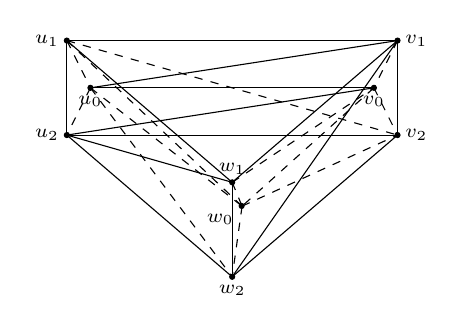
\begin{tikzpicture}[scale=0.6] %Complejo simplicial K homeomorfo al toro
            \draw (-1.5,3.5) -- (5.5,3.5);
            \draw[dashed] (-1.5,3.5) -- (-1.,2.5);
            \draw[dashed] (-1.,2.5) -- (-1.5,1.5);
            \draw (-1.,2.5) -- (5.,2.5);
            \draw[dashed] (5.5,3.5) -- (5.,2.5);
            \draw[dashed] (5.,2.5) -- (5.5,1.5);
            \draw (-1.5,1.5) -- (5.5,1.5);
            \draw (-1.5,3.5) -- (-1.5,1.5);
            \draw (5.5,3.5) -- (5.5,1.5);
            \draw[dashed] (5.,2.5) -- (2.209699462447651,-0.004690804599365735);
            \draw[dashed] (-1.,2.5) -- (2.209699462447651,-0.004690804599365735);
            \draw (2.,0.5) -- (-1.5,3.5);
            \draw (-1.5,1.5) -- (2.,-1.5);
            \draw (2.,0.5) -- (5.5,3.5);
            \draw (2.,-1.5) -- (5.5,1.5);
            \draw[dashed] (2.,0.5) -- (2.209699462447651,-0.004690804599365735);
            \draw (2.,0.5) -- (2.,-1.5);
            \draw[dashed] (2.209699462447651,-0.004690804599365735) -- (2.,-1.5);
            \draw[dashed] (-1.5,3.5) -- (5.5,1.5);
            \draw (-1.,2.5) -- (5.5,3.5);
            \draw (-1.5,1.5) -- (5.,2.5);
            \draw (-1.5,1.5) -- (2.,0.5);
            \draw (2.,-1.5) -- (5.5,3.5);
            \draw[dashed] (2.209699462447651,-0.004690804599365735) -- (5.5,1.5);
            \draw[dashed] (2.,0.5) -- (5.,2.5);
            \draw[dashed] (-1.,2.5) -- (2.,-1.5);
            \draw[dashed] (-1.5,3.5) -- (2.209699462447651,-0.004690804599365735);

            \begin{scriptsize}
                \draw [fill=black] (2.,-1.5) circle (1.5pt) node[anchor=north]{$w_{2}$};
                \draw [fill=black] (2.,0.5) circle (1.5pt) node[anchor=south]{$w_{1}$};
                \draw [fill=black] (2.2,0) circle (1.5pt) node[anchor=north east]{$w_{0}$};
                \draw [fill=black] (5.5,3.5) circle (1.5pt) node[anchor=west]{$v_{1}$};
                \draw [fill=black] (5.5,1.5) circle (1.5pt) node[anchor=west]{$v_{2}$};
                \draw [fill=black] (5.,2.5) circle (1.5pt) node[anchor=north]{$v_{0}$};
                \draw [fill=black] (-1.5,3.5) circle (1.5pt) node[anchor=east]{$u_{1}$};
                \draw [fill=black] (-1.5,1.5) circle (1.5pt) node[anchor=east]{$u_{2}$};
                \draw [fill=black] (-1.,2.5) circle (1.5pt) node[anchor=north]{$u_{0}$};
            \end{scriptsize}
        \end{tikzpicture}
        %
        \hspace{1cm}
        %
        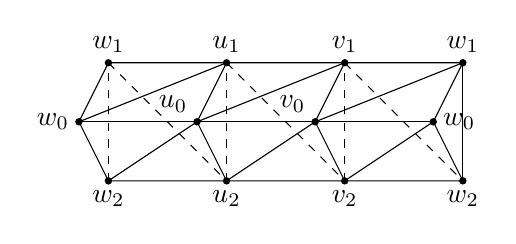
\begin{tikzpicture}[scale=1.5] %Representación del complejo simplicial K sin pegar extremos
            \coordinate (A) at (0,0);
            \coordinate (B) at (0,1);
            \coordinate (C) at (-1/4,1/2);

            \coordinate (D) at (1,0);
            \coordinate (E) at (1,1);
            \coordinate (F) at (3/4,1/2);

            \coordinate (G) at (2,0);
            \coordinate (H) at (2,1);
            \coordinate (I) at (7/4,1/2);

            \coordinate (J) at (3,0);
            \coordinate (K) at (3,1);
            \coordinate (L) at (11/4,1/2);

            \draw (A) -- (J) -- (L) -- (K) -- (B) -- (C) -- cycle;
            \draw (J) -- (K);
            \draw (C) -- (L);

            \draw[dashed] (A) -- (B);

            \draw (D) -- (F) -- (E);
            \draw[dashed] (D) -- (E);

            \draw (G) -- (I) -- (H);
            \draw[dashed] (G) -- (H);

            \draw (C) -- (E);
            \draw (A) -- (F) -- (H);
            \draw (D) -- (I) -- (K);
            \draw (G) -- (L);

            \draw[dashed] (B) -- (D);
            \draw[dashed] (E) -- (G);
            \draw[dashed] (H) -- (J);

            \filldraw (A) circle (0.75pt) node[anchor=north]{$w_{2}$};
            \filldraw (B) circle (0.75pt) node[anchor=south]{$w_{1}$};
            \filldraw (C) circle (0.75pt) node[anchor=east]{$w_{0}$};

            \filldraw (J) circle (0.75pt) node[anchor=north]{$w_{2}$};
            \filldraw (K) circle (0.75pt) node[anchor=south]{$w_{1}$};
            \filldraw (L) circle (0.75pt) node[anchor=west]{$w_{0}$};

            \filldraw (D) circle (0.75pt) node[anchor=north]{$u_{2}$};
            \filldraw (E) circle (0.75pt) node[anchor=south]{$u_{1}$};
            \filldraw (F) circle (0.75pt) node[anchor=south east]{$u_{0}$};

            \filldraw (G) circle (0.75pt) node[anchor=north]{$v_{2}$};
            \filldraw (H) circle (0.75pt) node[anchor=south]{$v_{1}$};
            \filldraw (I) circle (0.75pt) node[anchor=south east]{$v_{0}$};
        \end{tikzpicture}
    \end{center}
    En la segunda figura se muestra el complejo simplicial cortandolo en los vértices 
    $w_{0},w_{1}$ y $w_{2}$. Como los puntos de a ternas no son colineales vemos que cada simplice
    esta bien definido, además, cada simplice se pega bien. Por lo tanto $K$ esta bien definido.
    Por otro lado, triangulamos el cuadrado $\square:=[-1,1]^{2}$ del siguiente modo
    \begin{center}
        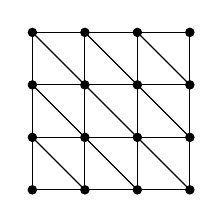
\begin{tikzpicture}[scale=2] %Triangulación del cuadrado
            \coordinate (A) at (0,0);
            \coordinate (B) at (1,0);
            \coordinate (C) at (1,1);
            \coordinate (D) at (0,1);
            
            \coordinate (E) at (1/3,0);
            \coordinate (F) at (2/3,0);
            
            \coordinate (G) at (1,1/3);
            \coordinate (H) at (1,2/3);

            \coordinate (I) at (2/3,1);
            \coordinate (J) at (1/3,1);

            \coordinate (K) at (0,2/3);
            \coordinate (L) at (0,1/3);

            \draw (A) -- (B) -- (C) -- (D) -- cycle;
            
            \draw (E) -- (J);
            \draw (F) -- (I);
            \draw (G) -- (L);
            \draw (H) -- (K);
            
            \draw (E) -- (L);
            \draw (F) -- (K);
            \draw (B) -- (D);
            \draw (H) -- (I);
            \draw (G) -- (J);

            \filldraw (A) circle (0.75pt);
            \filldraw (B) circle (0.75pt);
            \filldraw (C) circle (0.75pt);
            \filldraw (D) circle (0.75pt);

            \filldraw (K) circle (0.75pt);
            \filldraw (H) circle (0.75pt);
            
            \filldraw (L) circle (0.75pt);
            \filldraw (G) circle (0.75pt);

            \filldraw (E) circle (0.75pt);
            \filldraw (J) circle (0.75pt);
            \filldraw (1/3,2/3) circle (0.75pt);
            \filldraw (1/3,1/3) circle (0.75pt);

            \filldraw (F) circle (0.75pt);
            \filldraw (I) circle (0.75pt);
            \filldraw (2/3,2/3) circle (0.75pt);
            \filldraw (2/3,1/3) circle (0.75pt);
        \end{tikzpicture}
    \end{center}
    Donde cada vértice corresponde a un par ordenado con coordenadas en el conjunto 
    $\{0,1/3,2/3,1\}$, denotaremos por $V_{\square}$ al conjunto de vértices. Definimos el mapeo
    simplicial $f:V_{\square}\to V_{K}$ de modo que cada vértice en $V_{\square}$ se mapea a 
    $\abs{K}$ como en la siguiente figura,
    \begin{center}
        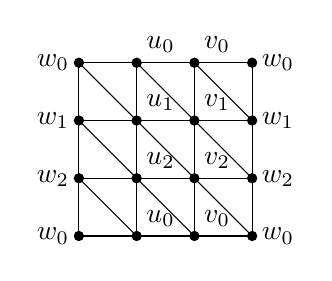
\begin{tikzpicture}[scale=2.2] %Mapeo simplicial del cuadrado al complejo simplicial K
            \coordinate (A) at (0,0);
            \coordinate (B) at (1,0);
            \coordinate (C) at (1,1);
            \coordinate (D) at (0,1);
            
            \coordinate (E) at (1/3,0);
            \coordinate (F) at (2/3,0);
            
            \coordinate (G) at (1,1/3);
            \coordinate (H) at (1,2/3);

            \coordinate (I) at (2/3,1);
            \coordinate (J) at (1/3,1);

            \coordinate (K) at (0,2/3);
            \coordinate (L) at (0,1/3);

            \draw (A) -- (B) -- (C) -- (D) -- cycle;
            
            \draw (E) -- (J);
            \draw (F) -- (I);
            \draw (G) -- (L);
            \draw (H) -- (K);
            
            \draw (E) -- (L);
            \draw (F) -- (K);
            \draw (B) -- (D);
            \draw (H) -- (I);
            \draw (G) -- (J);

            \filldraw (A) circle (0.75pt) node[anchor=east]{$w_{0}$};
            \filldraw (B) circle (0.75pt) node[anchor=west]{$w_{0}$};
            \filldraw (C) circle (0.75pt) node[anchor=west]{$w_{0}$};
            \filldraw (D) circle (0.75pt) node[anchor=east]{$w_{0}$};

            \filldraw (K) circle (0.75pt) node[anchor=east]{$w_{1}$};
            \filldraw (H) circle (0.75pt) node[anchor=west]{$w_{1}$};
            
            \filldraw (L) circle (0.75pt) node[anchor=east]{$w_{2}$};
            \filldraw (G) circle (0.75pt) node[anchor=west]{$w_{2}$};

            \filldraw (E) circle (0.75pt) node[anchor=south west]{$u_{0}$};
            \filldraw (J) circle (0.75pt) node[anchor=south west]{$u_{0}$};
            \filldraw (1/3,2/3) circle (0.75pt) node[anchor=south west]{$u_{1}$};
            \filldraw (1/3,1/3) circle (0.75pt) node[anchor=south west]{$u_{2}$};

            \filldraw (F) circle (0.75pt) node[anchor=south west]{$v_{0}$};
            \filldraw (I) circle (0.75pt) node[anchor=south west]{$v_{0}$};
            \filldraw (2/3,2/3) circle (0.75pt) node[anchor=south west]{$v_{1}$};
            \filldraw (2/3,1/3) circle (0.75pt) node[anchor=south west]{$v_{2}$};
        \end{tikzpicture}
    \end{center}
    Luego, $f$ induce una función continua continua de $\square$ a $\abs{K}$, que llamaremos $f$. 
    Notemos que $f$ es sobreyectiva en vértices, afirmamos que $f$ es sobreyectiva, en efecto, 
    dado $x\in\abs{K}$ se tiene que
    \begin{equation*}
        x=\sum t_{i}q_{i}\hhtext{entonces}x=f(y)=f\left(\sum t_{i}p_{i}\right)
    \end{equation*}
    donde $q_{i}\in\{u_{j},v_{j},w_{j}\}_{j=0}^{2}$ y tal que $f(p_{i})=q_{i}$. Como $\square$ es 
    compacto y $\abs{K}$ es Hausdorff, concluimos que $f$ es cociente.

    \vspace{2mm}
    Sea $\pi$ la proyección de $\square$ a $\mathbb{T}^{2}$. Veamos que $f$ es constante en las 
    fibras de $\pi$ y viceversa. Sea $t\in[0,1]$, notemos que $f(1,t)=f(0,t)$ y $f(t,0)=f(t,1)$, 
    lo que prueba la doble contención. Así, por propiedad universal de topología cociente, $f$ 
    induce una función continua $\rho:\abs{K}\to\mathbb{T}^{2}$ y del mismo modo $\pi$ induce una 
    función $h:\mathbb{T}^{2}\to\abs{K}$ también continua. Tenemos el siguiente diagrama,
    
    \vspace{2mm}
    \centerline{
        \xymatrix{
             & [0,1]^{2} \ar[ld]_{\pi} \ar[rd]^{f} \\
            \mathbb{T}^{2} \ar@{-->}[rr]^{h} & & \abs{K} \ar@{-->}@/^/[ll]^{\rho}
        }
    }
    Veamos que $h$ es la inversa de $\rho$. Sabemos que $\rho\circ f=\pi$ y $h\circ\pi=f$. Luego,
    sea $y\in\abs{K}$, existe $x\in\square$ tal que $y=f(x)$, así 
    $h\circ\rho(y)=h\circ\rho\circ f(x)=h\circ\pi(x)=f(x)=y$, por otro lado, 
    $\rho\circ h([x])=\rho\circ h\circ\pi(x)=\rho\circ f(x)=[x]$. Por lo tanto, $(K,\rho)$ es una 
    triangulación del toro. La característica de Euler es $V-E+F=9-27+18=0$.
\end{enumerate}

%\printbibliography % Quitar el comentado si quiero usar bibliografia

\end{document}
